\documentclass{standalone}

\usepackage{tikz}

\begin{document}

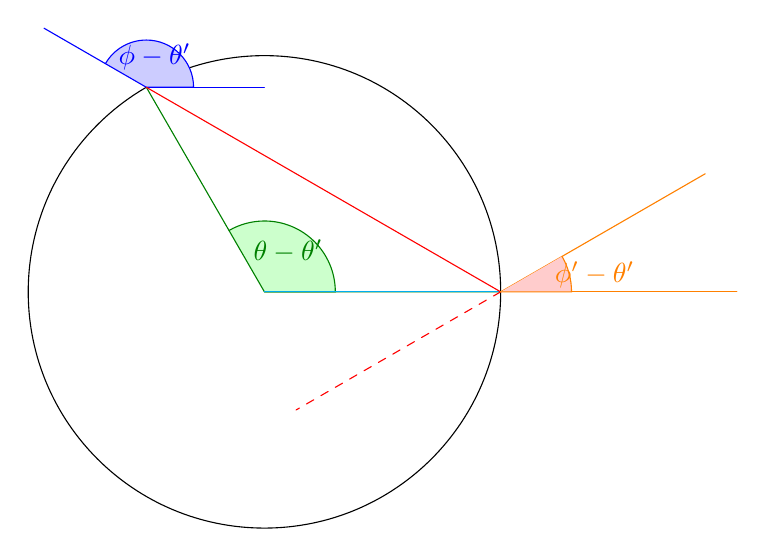
\begin{tikzpicture}[scale=3,cap=round]

    \colorlet{thetacolor}{green!50!black}
    \colorlet{phicolor}{blue}
    \colorlet{lcolor}{red}

    \draw (0,0) circle (1cm);

    \filldraw[fill=green!20,draw=thetacolor] (0,0) -- (.3,0) arc(0:120:3mm);
    \draw (60:2mm) node[thetacolor] {$\theta-\theta'$};

    \draw[thetacolor] (120:1cm) -- (0,0) -- (1cm, 0);

    \draw[cyan] (0:1cm) -- (0,0);

    \filldraw[fill=blue!20,draw=phicolor] (120:1cm) -- (-0.3,0.866 cm) arc(0:150:2mm);
    \draw (115:1.1cm) node[phicolor] {$\phi-\theta'$};

    \draw[phicolor] (120:1cm) -- +(-.433, .25);
    \draw[phicolor] (120:1cm) -- +(0.5cm,0);

    \draw[lcolor] (120:1cm) --  (0:1cm);

    \draw[lcolor,dashed] (0:1cm) -- +(-0.866,-0.5);
    \draw[orange] (0:1cm) -- +(0.866,0.5);
    \draw[orange] (0:1cm) -- +(1,0);

    \filldraw[fill=red!20,draw=orange] (0:1cm) -- +(.3,0) arc(0:30:3mm);
    \draw (3:1.4) node [orange] {$\phi'-\theta'$};

\end{tikzpicture}

\end{document}